\newcommand{\nocontentsline}[3]{}
\newcommand{\tocless}[2]{\bgroup\let\addcontentsline=\nocontentsline#1{#2}\egroup}


\newcommand{\SubAppendix}[1]{\tocless\section{#1}}

\appendix
\chapter{Appendix}

\SubAppendix{\acrfull{bamsoo} algorithm}
\label{ap:bamsoo_algo}

\begin{algorithm}[h]
    \caption{BamSOO}
    \label{algo:bamsoo}
    \KwIn{$\Omega$,$f$,$K$,$n_{\text{max}}$,$K_D$:}
    
    $x_{0,0} \gets \text{center}(\Omega)$ \;
    $g_{0,0} \gets f(x_{0,0})$ \;
    $\mathcal{T}_1 \gets \{x_{0,0}, g_{0,0}, \Omega\}$ \tcp{Initiate the tree}
    $f^+ \gets g_{0,0}$ \;
    $n \gets 1$,$t \gets 1$ \tcp{nodes and evaluation index}
    $\mathcal{D}_1 \gets \{x_{0,0}, g_{0,0}\}$ \tcp{list of evaluated points}
    
    \While{$t < n_{\text{max}}$}{
        $\nu_{\text{max}} \gets -\infty$ \;
        \For{$h \gets 0$ \KwTo $\text{depth}(\mathcal{T}_n)$}{
            $j \gets \arg\max_{j \in \{j \mid (h,j) \in L_n\}} g_{h,j}$ \;
            \If{$g_{h,j} > \nu_{\text{max}}$}{
                $\Omega_{h+1,j+1}, \dots, \Omega_{h+1,j+K} \gets \text{section}(\Omega_{h,j}, K)$ \;
                \For{$i \gets 1$ \KwTo $K$}{
                    $\mu, \sigma \gets \text{GP}(\mathcal{D}_t, K_D)$ \;
                    $N \gets N+1$ \;
                    $x_{h+1,j+i} \gets \text{center}(\Omega_{n})$ \;
    
                    \If{$\mathcal{UCB}(x_{h+1,j+i}, \mu, \sigma) \geq f^+$}{
                        $g_{h+1,j+i} \gets f(x_{h+1,j+i})$ \;
                        $t \gets t+1$ \;
                    }\Else{
                        $g_{h+1,j+i} \gets \mathcal{LCB}(x_{h+1,j+i}, \mu, \sigma)$ \;
                    }
    
                    \If{$g_{h+1,j+i} > f^+$}{
                        $f^+ \gets g_{h+1,j+i}$ \;
                    }
                    $n \gets n+1$ \;
                    $\mathcal{T}_n \gets \{(x_{h+1,j+i}, f_{h+1,j+i}, \Omega_{h+1,j+i})\}$ \;
                }
                $\nu_{\text{max}} \gets g_{h,j}$ \;
            }
        }
    }
    \Return best of $x_{h,j}, g(x_{h,j})$ \;
    \end{algorithm}

\SubAppendix{Internship offer}
\label{ap:internship}
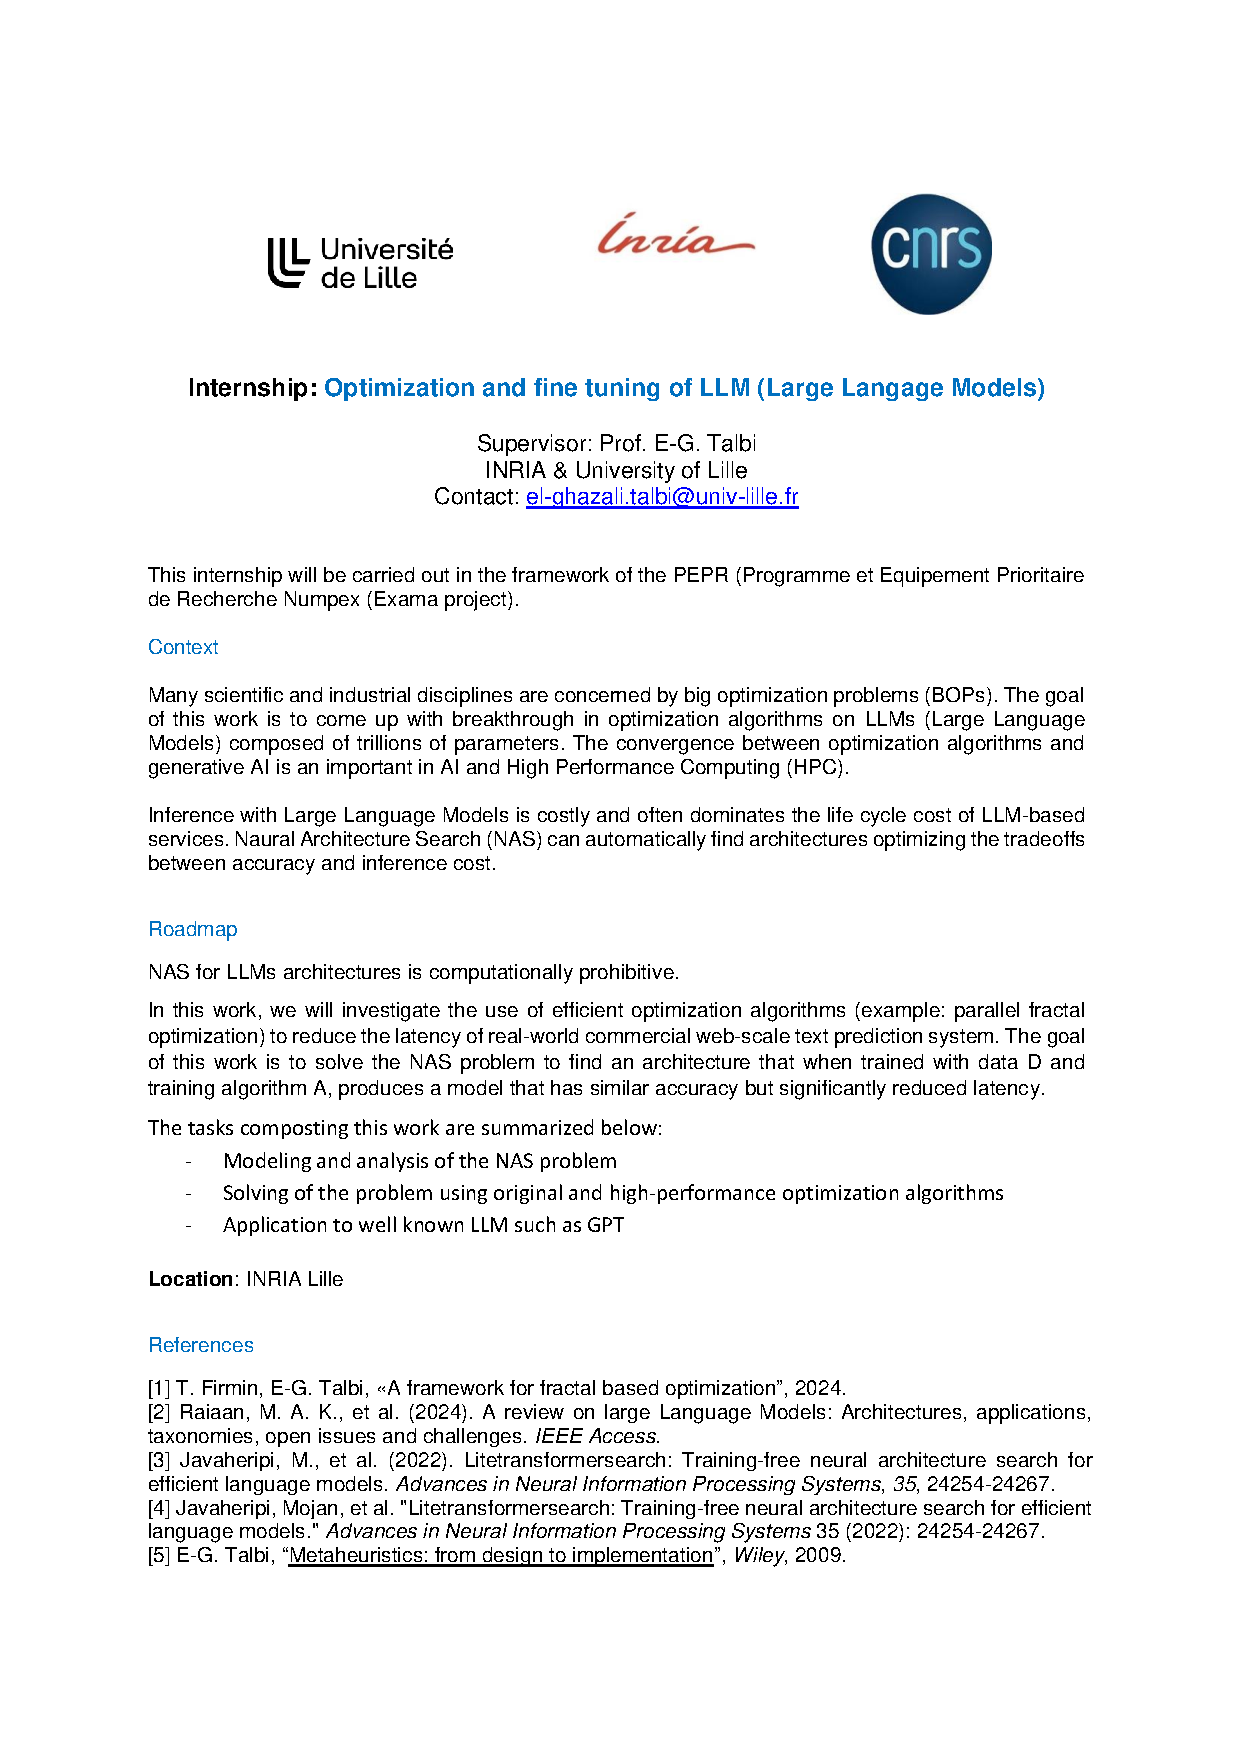
\includepdf[pages=-]{latex-files/annexes/Internship.pdf}

\SubAppendix{\acrfull{lhs} algorithm}
\label{ap:lhs_algo}

\begin{algorithm}[H]
    \SetAlgoLined
    \KwIn{Number of samples $N$, Number of dimensions $D$}
    \KwOut{$N \times D$ matrix of sampled points}
    
    Initialize an empty matrix $M$ of size $N \times D$\;
    
    \For{each dimension $i \in \{1, 2, \dots, D\}$}{
        Divide the range $[0, 1]$ into $N$ equally spaced intervals\;
        Shuffle the interval indices randomly\;
        \For{each sample $j \in \{1, 2, \dots, N\}$}{
            Pick a random value $x$ within the $j$-th interval\;
            Assign $x$ to $M[j][i]$\;
        }
    }
    \Return{$M$}
    \caption{Latin Hypercube Sampling Algorithm}
\end{algorithm}